\documentclass{beamer}
\usepackage[utf8x]{inputenc} %kodovaní UTF-8
\usepackage{ucs} %kodovani unicode
\usepackage[czech]{babel} %podpora cestiny
\usepackage[T1]{fontenc} %pouzij variantu pisma T1 (hacky, carky)
\usepackage{graphicx}
%\usepackage[dvipsnames]{xcolor} %barvy textu

% >>>>>>> Šablona pro prezentaci <<<<<<<
\usetheme{Frankfurt}
\useinnertheme{circles}
\usepackage{subfigure}
\usefonttheme{professionalfonts}
\usepackage{lmodern} % fonts in a LaTeX document
\usepackage{color}
\definecolor{mygray}{rgb}{0.5,0.5,0.5}

\usepackage{movie15} %Pro video
\usepackage{geometry}

%Figure numbering
\setbeamertemplate{caption}[numbered]

%Odstranění navigační lišty a přidání čísle slajdů
\beamertemplatenavigationsymbolsempty

%\addtobeamertemplate{navigation symbols}{}{%
%    \usebeamerfont{footline}%
%    \usebeamercolor[fg]{footline}%
%    \hspace{1em}%
%    \insertframenumber/\inserttotalframenumber
%}

\makeatletter
\setbeamertemplate{navigation symbols}{
    \ifbeamer@inappendix%
  \else%
    \usebeamerfont{footline}%
        \usebeamercolor[fg]{footline}%
    \insertframenumber\,/\,\insertmainframenumber%
  \fi%
}
\makeatother

% >>>>>>> Funkce <<<<<<<



% >>>>>>> Informace o práci <<<<<<<
\def\uv#1{\char92\relax #1\char34\relax}
%%%%%%%%%%%%%%%%%%%%%%%%%%%%%%%%%%%%%%%%%%%%%%%%%%%%%%%%%%%%%%%%%%
\newcommand\FirstName{Jan}
\newcommand\FirstNameAbbreviated{F}
\newcommand\LastName{Závorka}
\newcommand\Email{zavorja4@fel.cvut.cz}
\newcommand\DissertationTitle{Interaktivní hra využívající IoT prostředky}
\newcommand\Department{Katedra radioelektroniky}
\newcommand\Faculty{Fakulta elektrotechnická}
\newcommand\University{České vysoké učení technické v Praze \\[.3em] 
\includegraphics[width=3cm]{img/LogoCVUT.pdf}}
\newcommand\FacultyAndUniversityAbbr{FEL ČVUT}
%%%%%%%%%%%%%%%%%%%%%%%%%%%%%%%%%%%%%%%%%%%%%%%%%%%%%%%%%%%%%%%%%%
\subject{SUBJECT}
\author[\FirstNameAbbreviated. \LastName]{\FirstName{} \LastName \\ {\color{mygray}\Email}}
\title{\DissertationTitle}
%\titlegraphic{
\includegraphics[width=1.5cm]{img/LogoCVUT.pdf}}
\institute[\FacultyAndUniversityAbbr]{\Department\\ \Faculty\\ \University \\[1em]}
\date{\today}
%\logo{
\includegraphics[width=4cm]{img/LogoCVUT.pdf}}




\begin{document}
%\setcounter{numberoframes}{\inserttotalframenumber}
{
\beamertemplatenavigationsymbolsempty
\begin{frame}[plain]
\maketitle
\end{frame}
\addtocounter{framenumber}{-1}
}
%
\section{Obsah}
\begin{frame}[allowframebreaks]
\frametitle{Obsah}
\tableofcontents
\end{frame}

\section{Cíl práce}
\begin{frame}
\frametitle{Cíl práce}
Demonstrační zařízení:
\begin{itemize}
\item Energeticky nenáročná zařízení
\item Forma jednoduché hry
\item Komunikace po síti 
\end{itemize}
\end{frame}

\section{Realizace}
\begin{frame}
\frametitle{Realizace}
 \begin{itemize}
 \item Hra piškvorky
 \item Platforma Arduino 
\includegraphics[height=0.4cm]{img/Arduino.png}
 	\begin{itemize}
 		\item Server - řízení hry
 		\item Klient - interakce s uživatelem
 	\end{itemize}
 \item 3D tisk krabiček (PLA)
 \item Komunikace po lokální síti (centrální prvek switch)
 
 \pause
 \begin{figure}
 \centering
 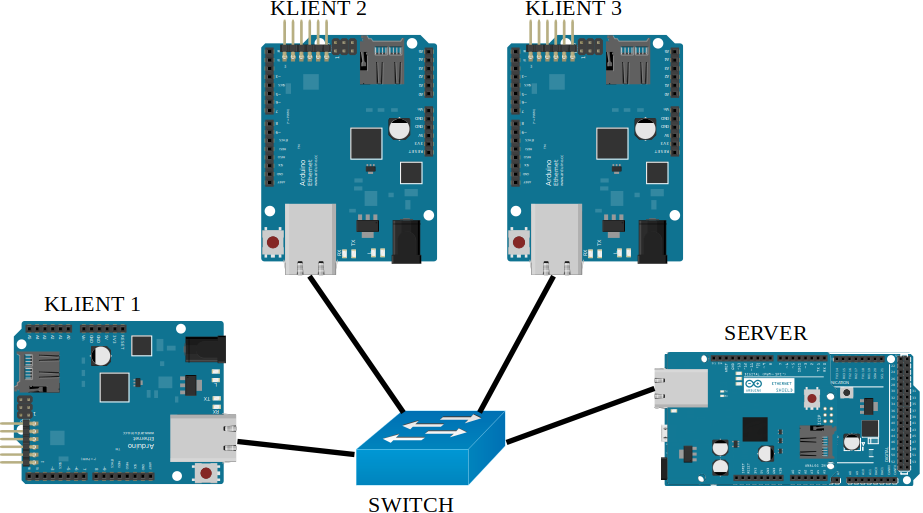
\includegraphics[width=7.5cm]{img/schema_net.png}
 \caption{Schéma zapojení jednotlivých zařízení do sítě}
 \end{figure}
 \end{itemize}
\end{frame}

\begin{frame}
\frametitle{Realizace - server}
\begin{columns}[c]
 \column{.5\textwidth}
	\begin{figure}
		\centering
		
\includegraphics[width=\textwidth]{img/server_realizace.jpg}
		\caption{Fotografie serveru}
	\end{figure}
%
 \column{.5\textwidth}
	\only<1>{
 		\begin{itemize}
 			\item Arduino Due + Ethernet shield + vlastní DPS
 			\item RJ-45 konektor
 			\item Souosý napájecí konektor (6~-~16~V)
 			\item Indikace stavu pomocí svítivé diody
 			\item Ovládání pomocí tlačítek a sériového rozhraní
 		\end{itemize}
	} 	
 	\only<2>{
		\refstepcounter{framenumber}
		
 		{\color{green} Zelené tlačítko:} Spuštění hry, 
 		
 		\hspace{2.5cm} posun hráče
 		
		{\color{red} Červené tlačítko:} Zastavení hry 	
		\begin{table}
			\centering
			\caption{Stavy svítivé diody}
			\includegraphics[width=\textwidth]{img/serverLED.png}
		\end{table}
	}
\end{columns}
\end{frame}

\begin{frame}
\frametitle{Realizace - klient}
\begin{columns}[c]
 \column{.5\textwidth}
	\begin{figure}
		\centering
		
\includegraphics[width=\textwidth]{img/client_realizace.jpg}
		\caption{Fotografie klienta}
	\end{figure}
%
 \column{.5\textwidth}
 		\begin{itemize}
 			\item Arduino Ethernet
 			\item RJ-45 konektor
 			\item Souosý napájecí konektor (6~-~20~V)
 			\item $2,4^{\prime\prime}$ barevný displej
 			\item Rezistivní dotyková plocha
 		\end{itemize}	
\end{columns}
\end{frame}

\begin{frame}
\frametitle{Video ukázka}
%\includemedia[
%     width=6cm,height=6cm,
%     activate=pageopen,
%     addresource=video/Guinness.mp4,
%     flashvars={
%         source=video/Guinness.mp4
%        &autoPlay=true
%     } 
%]{}{VPlayer.swf}
%\includemovie[poster,text={\small(Loading Video...)}]{6cm}{4cm}{video/Guinness.mp4}
Video přidat sem
\end{frame}


\section{Diskuze}
\begin{frame}
\begin{center}
\vspace*{1cm}
{\bf Děkuji za pozonost!}\\
\vspace*{1.2cm}
{\bf\Large \FirstName{} \LastName{}}\\
{\tt \Email} \\[1em]
Stránka projektu na GitHubu: \\
\url{https://github.com/janzavorka/BP_PROJ}
\vspace*{1cm}
\end{center}
\end{frame}

\appendix

\section{Otázka 1}
\begin{frame}
\frametitle{Využití PoE (Power over Ethernet)}
Možnosti pro klientské zařízení:
\begin{itemize}
	\item deska Arduino Ethernet má přípravu pro PoE (existují varianty osazeným PoE modulem)
	\only<2->{
		\item Modul s výstupním napětí 5~V nebo 12~V (resp. 5,5~V a 12,5~V)
		\item Výstup PoE modulu napojen na vstup lin. stabilizátoru Arduina
	}
\end{itemize}
\only<1>{
	\begin{figure}
		\centering
		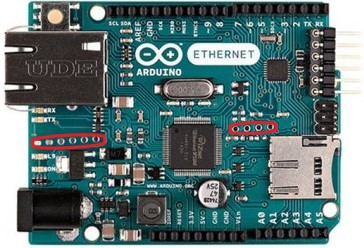
\includegraphics[width=.7\textwidth]{img/ardEth_nopoe.jpg}
		\caption{Arduino Ethernet s označenými piny pro připojení PoE modulu}
	\end{figure}
}

\only<2>{
	\refstepcounter{figure}
	\begin{figure}
		\centering
		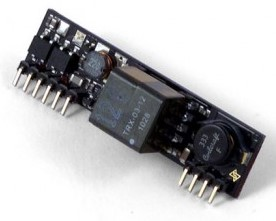
\includegraphics[width=.4\textwidth]{img/poe.jpg}
		\caption{Modul PoE pro Arduino}
	\end{figure}
}

\only<3->{
Problémy:
\begin{itemize}
	\item 5~V modul - úbytek na lin. stab. $\approx 0,8~V$: reference pro displej
	\item 12~V modul - stabilizátor nezvládá velký ztrátový výkon (odběr 350~mA)
\end{itemize}
}
\end{frame}

\begin{frame}
\frametitle{Využití PoE (Power over Ethernet)}
Pro server:
\begin{itemize}
	\item Ethernet shield s PoE
	\item Nutný switch s podporou PoE
	\item PoE čistě pro server zbytečné
\end{itemize}
\end{frame}

\end{document}